\documentclass{scrartcl}
\usepackage[mathletters]{ucs}
\usepackage[utf8x]{inputenc}
\usepackage{amssymb}
\usepackage{amsmath}
\usepackage[usenames]{color}
\usepackage{hyperref}
\usepackage{wasysym}
\usepackage{graphicx}
\usepackage[normalem]{ulem}
\usepackage{enumerate}

\usepackage{listings}

\lstset{ %
basicstyle=\footnotesize,       % the size of the fonts that are used for the code
showspaces=false,               % show spaces adding particular underscores
showstringspaces=false,         % underline spaces within strings
showtabs=false,                 % show tabs within strings adding particular underscores
frame=single,                   % adds a frame around the code
tabsize=2,                      % sets default tabsize to 2 spaces
breaklines=true,                % sets automatic line breaking
breakatwhitespace=false,        % sets if automatic breaks should only happen at whitespace
}


\title{Masterproef Tool Wear Inspection - Meeting3 TJ}
\date{dinsdag 08 december 2020}
\author{}

\begin{document}

\maketitle

		\section{Masterproef Tool Wear Inspection - Meeting3 TJ}

Created vrijdag 20 november 2020



Meeting 04/11/2020



Tom Jacobs



Verschillende soorten materialen voor maximaal reflecterende golflengte?

	Allemaal hetzelfde materiaal binnenin, buitenste laag enkel verschillend
	
	Voornamelijk carbide als binnenste materiaal; zien met 1 foto op wavelength voor carbide of het er goed uitkomt
	
	\href{https://www.equipment-news.com/the-right-grade-creates-the-right-tool-selecting-tool-materials/}{https://www.equipment-news.com/the-right-grade-creates-the-right-tool-selecting-tool-materials/}
	
	

	 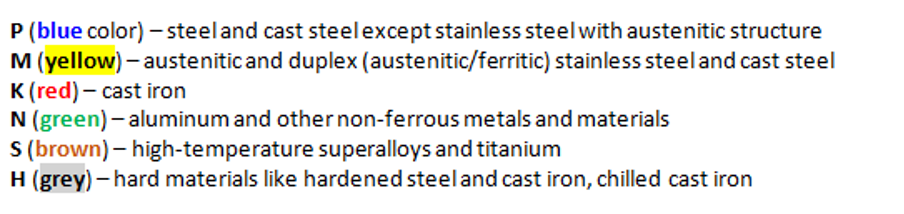
\includegraphics[width=4.166667in, keepaspectratio=true]{./Masterproef_Tool_Wear_Inspection_-_Meeting3_TJ/Types_sterkte_plaatjes.png}
	
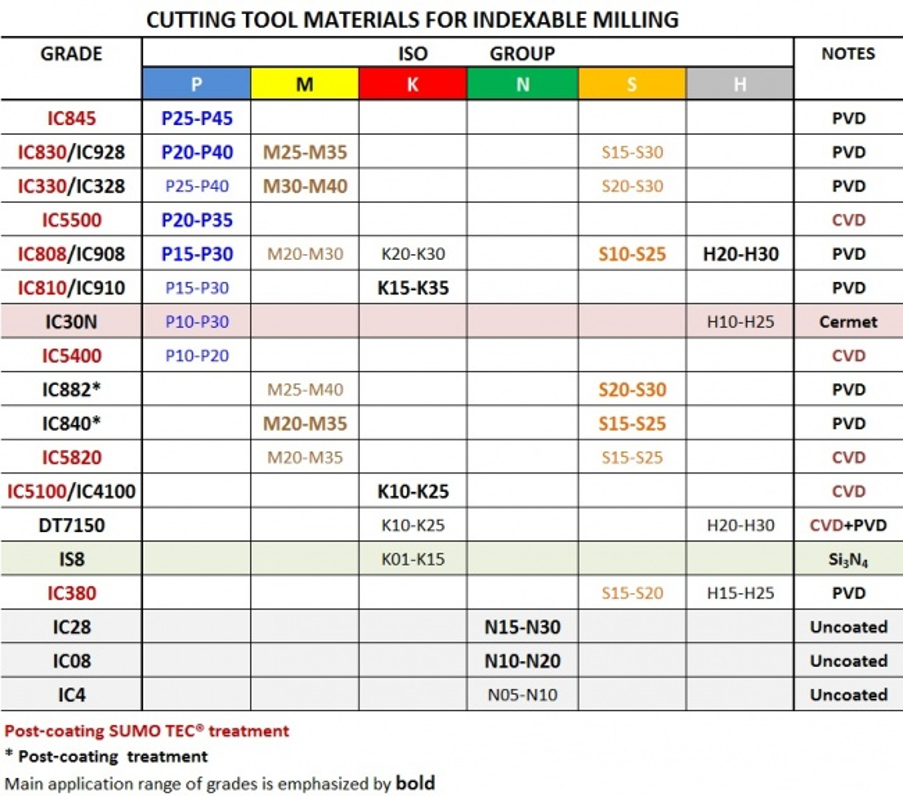
\includegraphics[width=4.166667in, keepaspectratio=true]{./Masterproef_Tool_Wear_Inspection_-_Meeting3_TJ/plaatjes_nummers.png}



Wat slijt er af?

	Is het afgesleten wanneer de coating weg is
	
		Coating slijt eerst af, daarna wordt het materiaal binnenin afgesleten
		
	Of wordt er gewoon een stukje van de coating afgesleten
	


De nauwkeurigheid van de frees -\textgreater{} om te vergelijken met de stappenmotor die op 0,106° nauwkeurig zal bewegen 

	Niet indexeerbaar of te draaien, desnoods uit frees nemen en in houder zetten om de foto te nemen, dus zelf ook niet te nauwkeurig werken.
	
	





Heeft u enkele voorbeelden van de verschillende slijtage types van de plaatjes?

	4 hoofd klassen, moeilijk om van allemaal een voorbeeld te vinden
	




Hoe ver moet gekeken worden op de kop en op de zijkant?

	Op de hoek zal steeds de slijtage zichtbaar zijn.
	
	

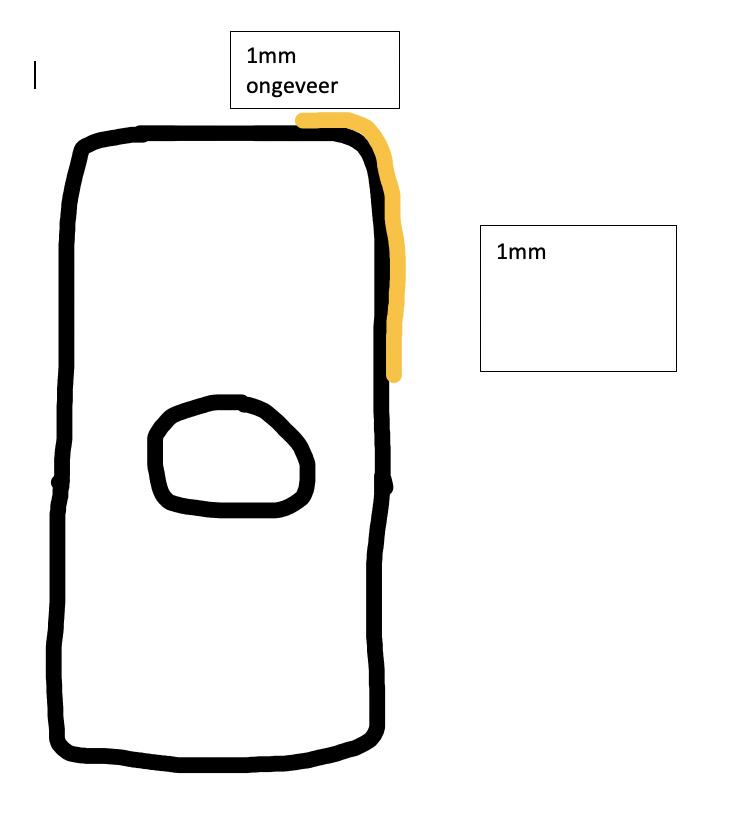
\includegraphics[width=4.166667in, keepaspectratio=true]{./Masterproef_Tool_Wear_Inspection_-_Meeting3_TJ/Screenshot 2020-11-20 at 15.20.56.png}



Extra metric toevoegen die de oppervlakte geeft van de fout, niet enkel de afstand die gegeven is voor test set. 

	Gewoon lichte pixels berekenen







\end{document}
